\chapter{Workshop and user testing}

\epigraph{Yeah you wanted a hit \\ but tell me \\ where's the point in it?}{You Wanted a Hit \\ LCD Soundsystem, 2010}

In the past I have taught several classes and crash courses of software of arts, and I used this experience to create a workshop for teaching Tiny Trainable Instruments. Teaching with this thesis project was conceived as a way of user testing and releasing to a wider non-academic audience. In this chapter I explain the workshops's design process, the feedback received from the students, and the challenges faced.

\section{Workshop design}

The Tiny Trainable Instruments workshop primary audience is artists and educators with no previous technical knowledge of programming, \acrshort{ML}, or microcontrollers. It is a hands-on class, where students build their own Tiny Trainable Instruments, create their own databases, and train their own \acrshort{ML} models.

The workshop consists of two sessions of two hours each, taught in two consecutive days for a total of four hours. The first session is focused on installation of the software, connecting the hardware components, and instruments using the color input. The second session is about capturing data and training models, for gesture and speech detection. During both sessions we use different outputs, including serial for text, servo for movement, and buzzer for sound.

This workshop was taught three times, the first two in English for people based in the U.S.A., and the third one in Spanish for people based in Chile. Each workshop had between six and seven students, for a total of twenty students. The three workshops were taught in the span of ten days, and each iteration informed the next one. Between sessions I tweaked the documentation, the class script, and the different code examples to make them easier to understand.

The workshop is designed to be taught virtually or presentially. The students require a laptop computer, internet connection, and a bill of materials for building the Tiny Trainable Instruments. To eliminate cost barriers, I applied and was awarded a generous grant of 2,000.00 USD from the \acrlong{CAMIT}. This funding was used to pay for all the materials and shipping for the 20 participants, who signed up, attended for free, and kept the materials to keep on building Tiny Trainable Instruments on their own.

The workshop also complied with the requirements and was approved by the \acrshort{MIT} \acrfull{COUHES}. This workshop posed a minimal risk to the participants, since effortes were made so that the students wouldn't share any data with me, and so that they were always in control of their privacy. The materials for building the Tiny Trainable Instruments are safe, low voltage, and used in similar educational settings, so all requirements were met for participants' safety. Additionally, the teaching was conducted over videoconferencing software, to ensure all health protocols were respected.

\section{Workshop promotion}

For promoting the workshop I collaborated with designer Renata Gaui \cite{website-renata-gaui}, who designed the bilingual workshop flyers in English and Spanish. I posted these flyers on my Instagram and Twitter accounts, and they were shared by  artists, designers, educators, and activists from different communities in U.S.A. and Chile.

\begin{figure}[ht]
  \centering
  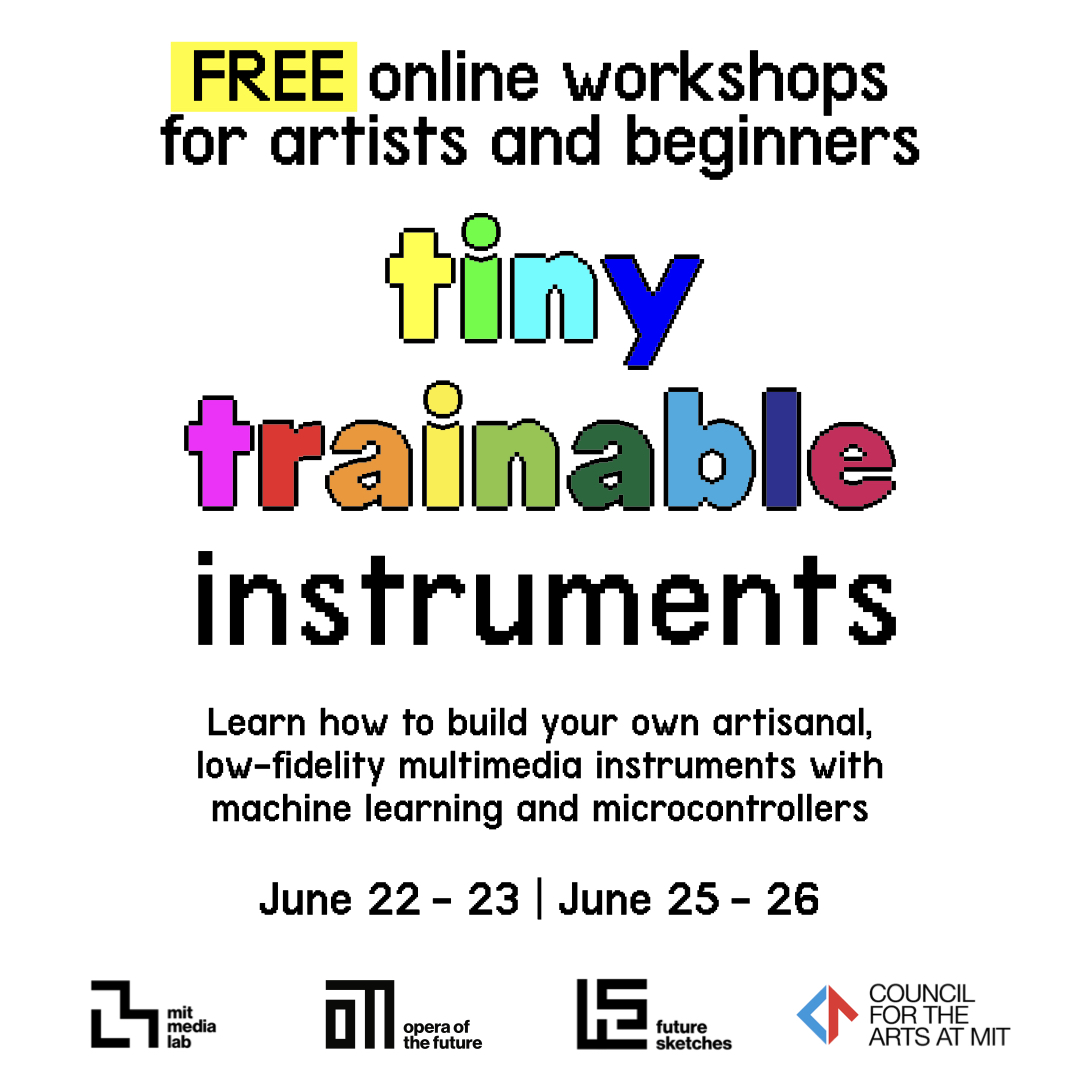
\includegraphics[width=0.75\linewidth,height=0.35\textheight,keepaspectratio]{images/workshop-en-1.jpg}
  \caption{Workshop flyer cover, in English}
  \caption*{Flyer by Renata Gaui}
  \label{fig:workshop-english-flyer-page-1}
\end{figure}

% \begin{figure}[ht]
%   \centering
%   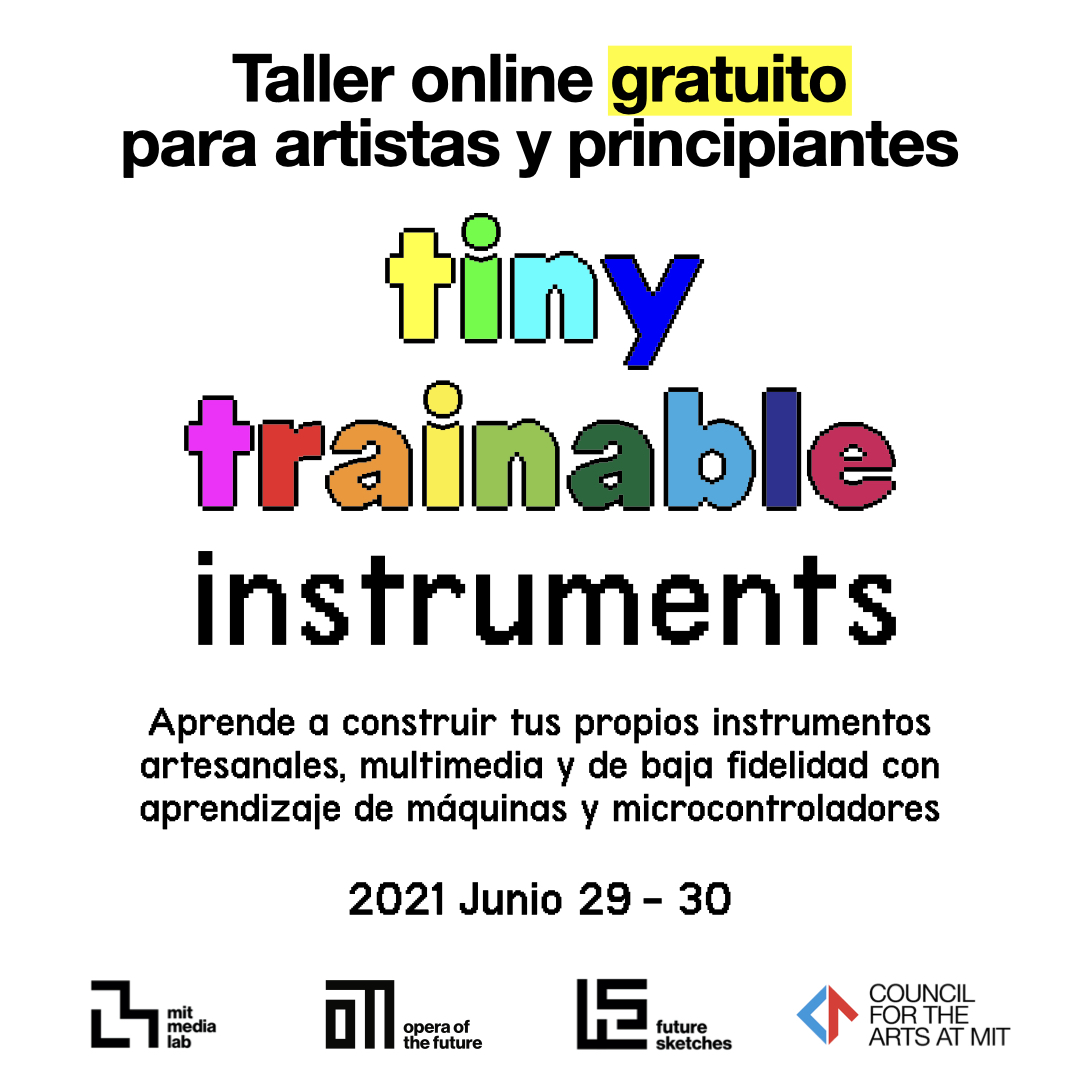
\includegraphics[width=0.75\linewidth,height=0.35\textheight,keepaspectratio]{images/workshop-es-1.jpg}
%   \caption{Workshop flyer cover in Spanish}
%   \caption*{Flyer by Renata Gaui}
%   \label{fig:workshop-spanish-flyer-page-1}
% \end{figure}

The flyers highlighted the multimedia and political orientation of Tiny Trainable Instruments, explaining that in the workshop people would learn how to use \acrshort{ML} with different inputs, including color, gesture and speech, to control different artistic outputs, including text over serial communication, buzzer sounds, and motor movement. The flyer also included a picture of a Tiny Trainable Instruments prototype, made with the Arduino microcontroller on a breadboard, jumper wires, a servo motor, and masking tape, to convey an artisanal and welcoming environment for beginners.

% \begin{figure}[ht]
%   \centering
%   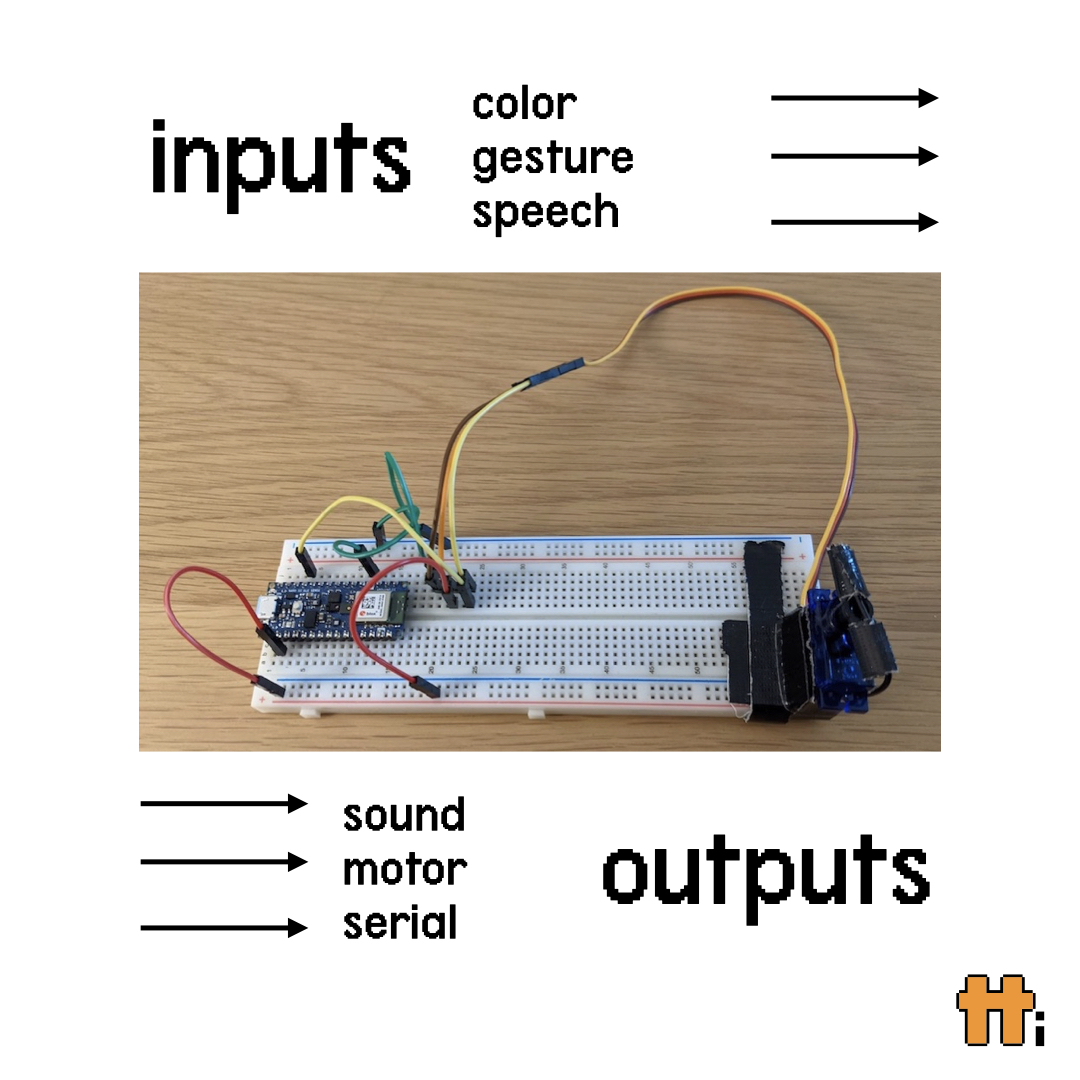
\includegraphics[width=0.75\linewidth,height=0.35\textheight,keepaspectratio]{images/workshop-en-2.jpg}
%   \caption{Workshop flyer multimedia output in English}
%   \caption*{Flyer by Renata Gaui}
%   \label{fig:workshop-english-flyer-page-2}
% \end{figure}

\begin{figure}[ht]
  \centering
  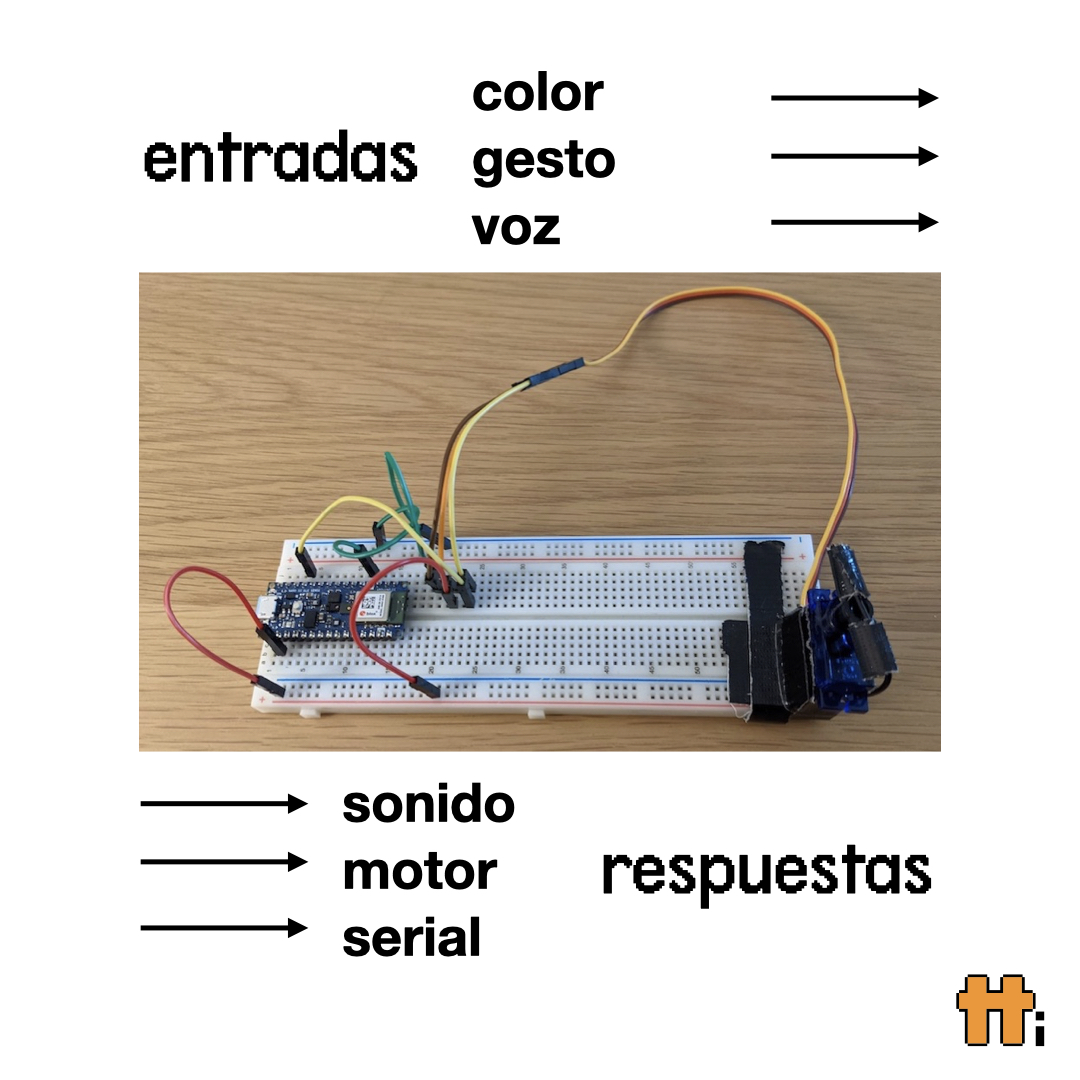
\includegraphics[width=0.75\linewidth,height=0.35\textheight,keepaspectratio]{images/workshop-es-2.jpg}
  \caption{Workshop flyer multimedia inputs and outputs, in Spanish}
  \caption*{Flyer by Renata Gaui}
  \label{fig:workshop-spanish-flyer-page-2}
\end{figure}

More than ninety people signed up for the twenty available spots. I consider this open call to be succesful, since it reached people who I didn't know at all who were entushiastic about this project. I picked the twenty students, so that I could have a diverse crowd, including artists, designers, musicians, programmers, educators, and activists. I included some acquaintances and former students, with the hope to get deeper feedback from them during and after the workshop. It also helped me to have more confidence while teaching on this new virtual format, and after a one year hiatus of organizing workshops.

\section{Workshop logistics}

The three workshops were taught respectively on June 22-23, June 25-26, and June 29-30 2021. Before each one, the participants were sent a basic kit for building Tiny Trainable Instruments, including these six materials: Arduino microcontroller, breadboard, jumper wires, USB cable, buzzer, servo motor.

The first four materials are needed for any Tiny Trainable Instruments, and the last two were picked for outputting sound and movement, to appeal to a wide audience of artists. They were also selected over because of their easy wiring and cheap cost, compared to the other outputs supported by the software library.

The Arduino microcontroller can be acquired from the Arduino online store, or from other electronics distributors. The rest of the materials are available on Adafruit, picked because of its focus on being an electronics store for artists and beginners. For the thirteen students in the U.S.A. I acquired the materials from sellers Arduino and Adafruit, and then shipped them to their addressses their kits via \acrfull{USPS}.

\begin{figure}[ht]
  \centering
  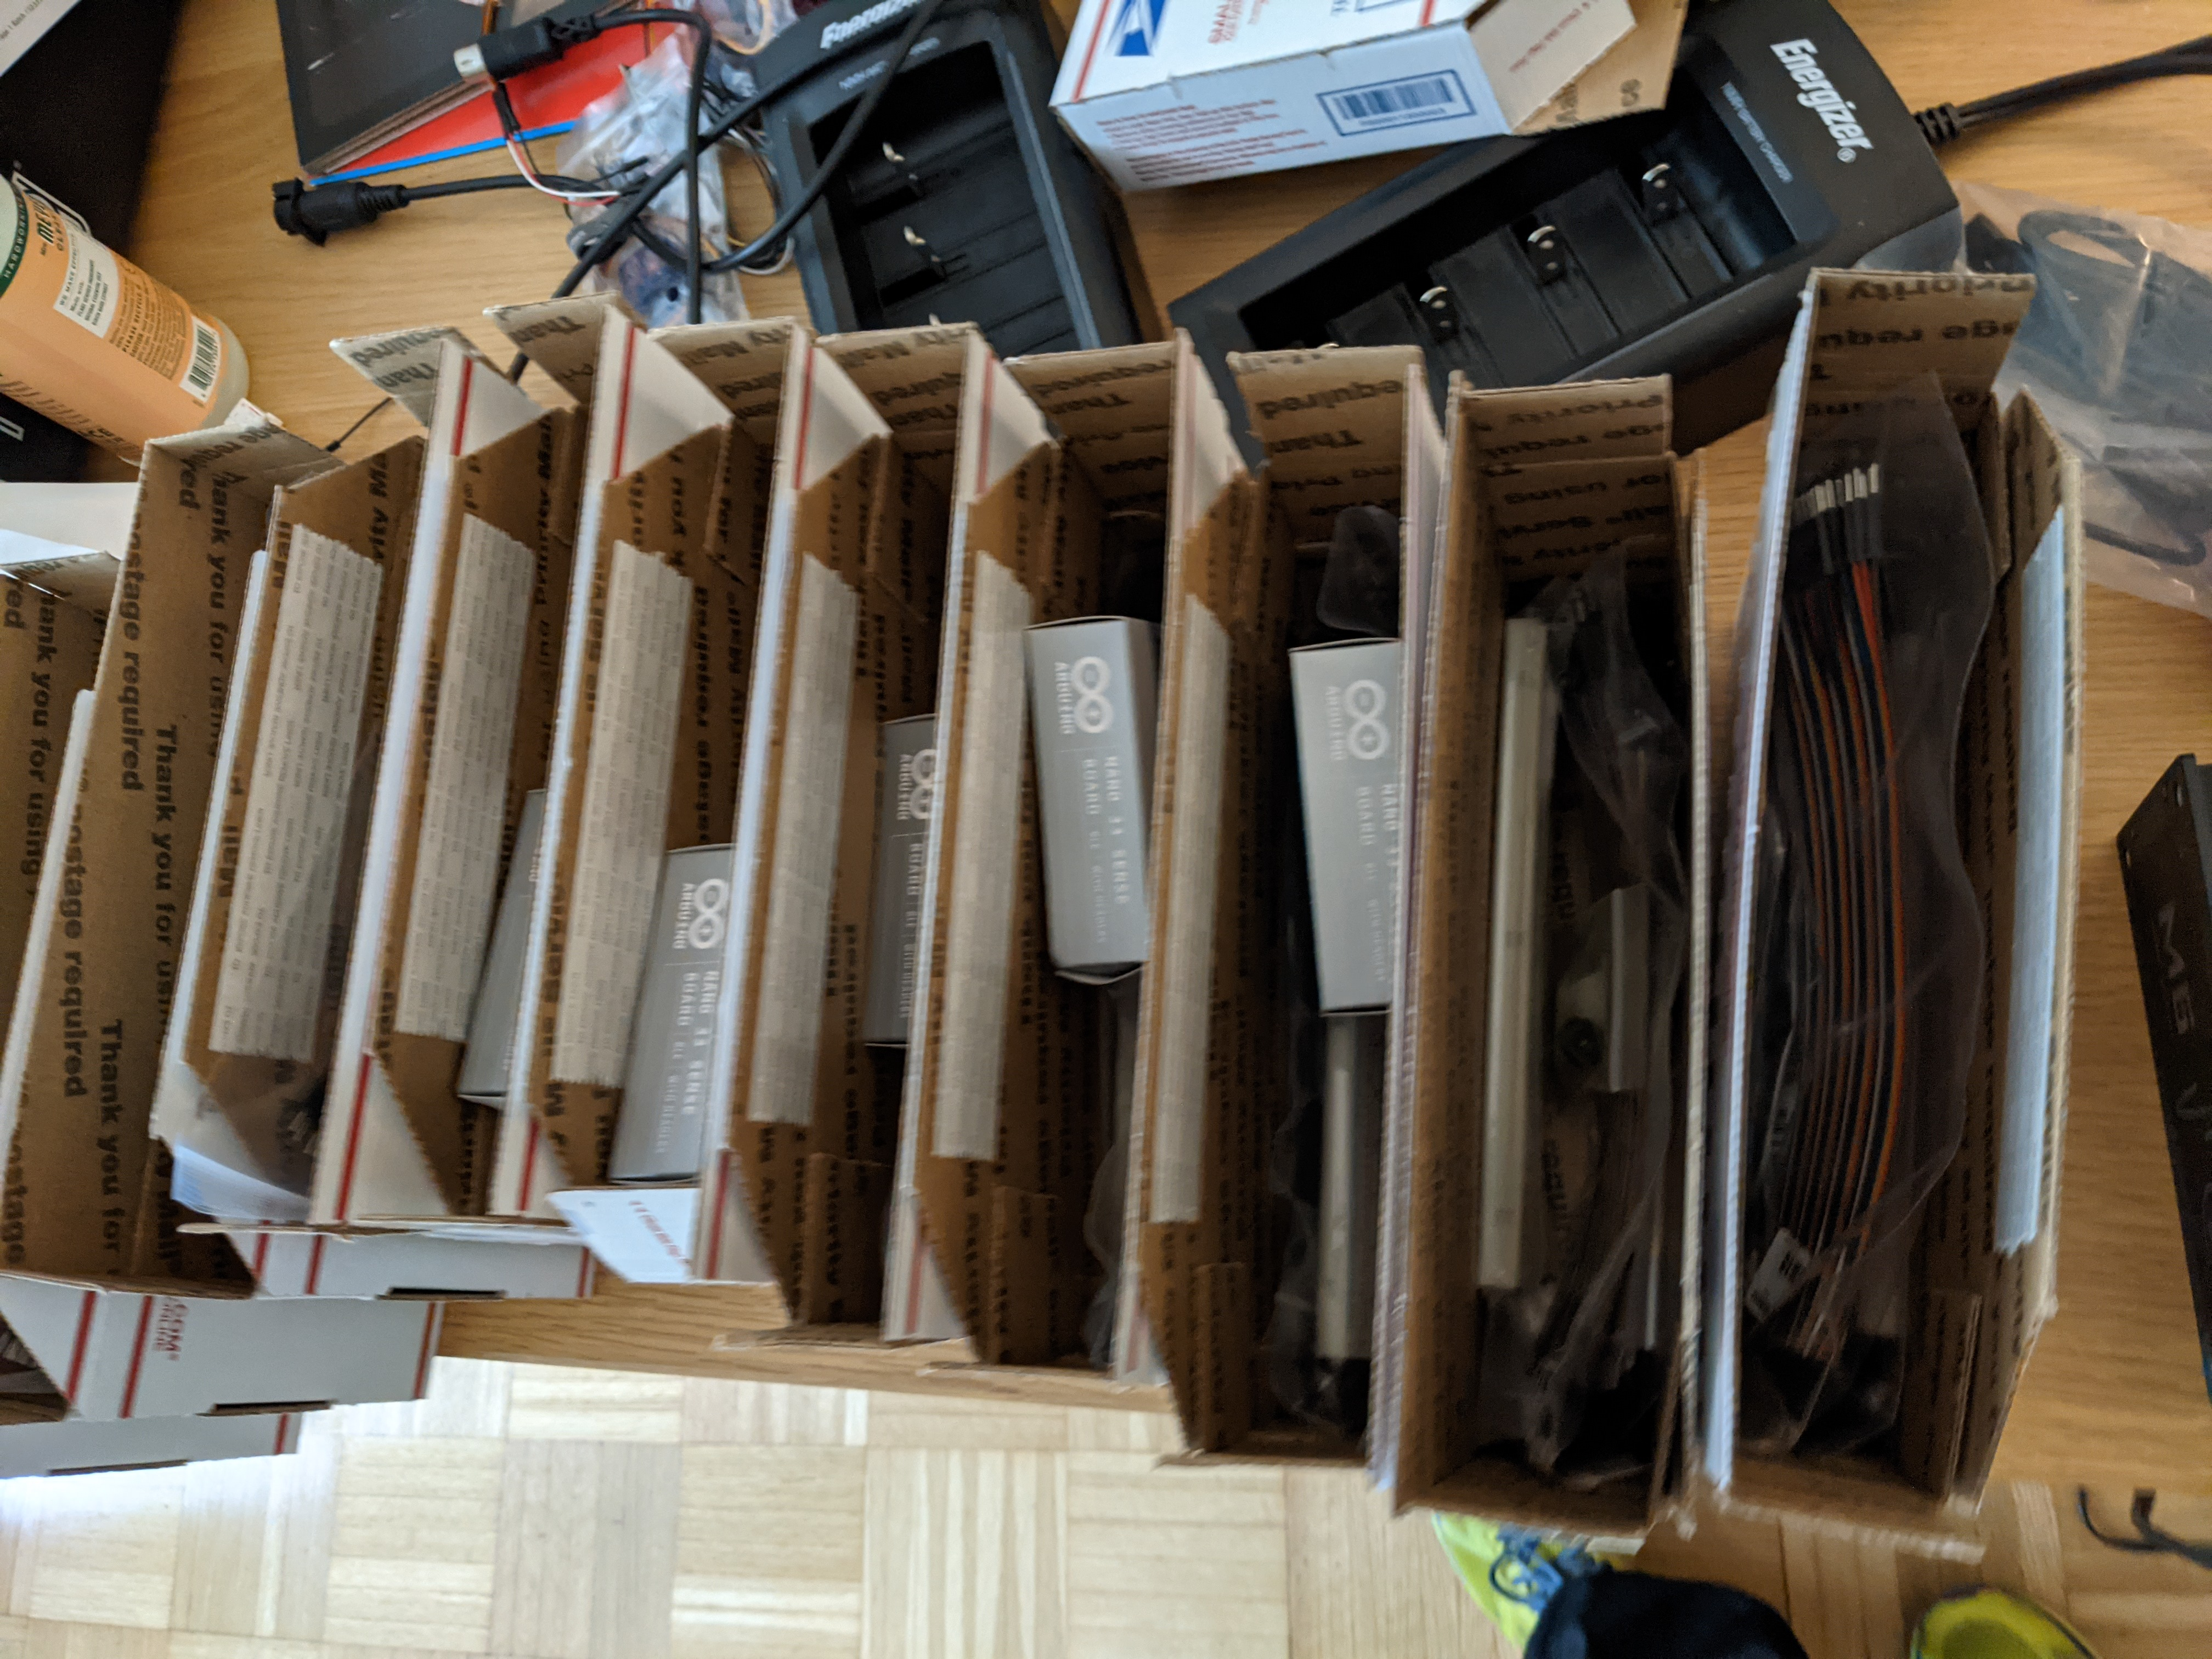
\includegraphics[width=0.75\linewidth,height=0.25\textheight,keepaspectratio]{images/workshop-packages.jpg}
  \caption{Workshop packages for the students in U.S.A.}
  \caption*{Picture by myself}
  \label{fig:workshop-packages-usa}
\end{figure}

For the seven students in Chile, I acquired the materials from the same vendor, and shipped them to my mother's home in Chile. She also sorted them in kits and then distributed them to the participants, via pickup or mail.

\begin{figure}[ht]
  \centering
  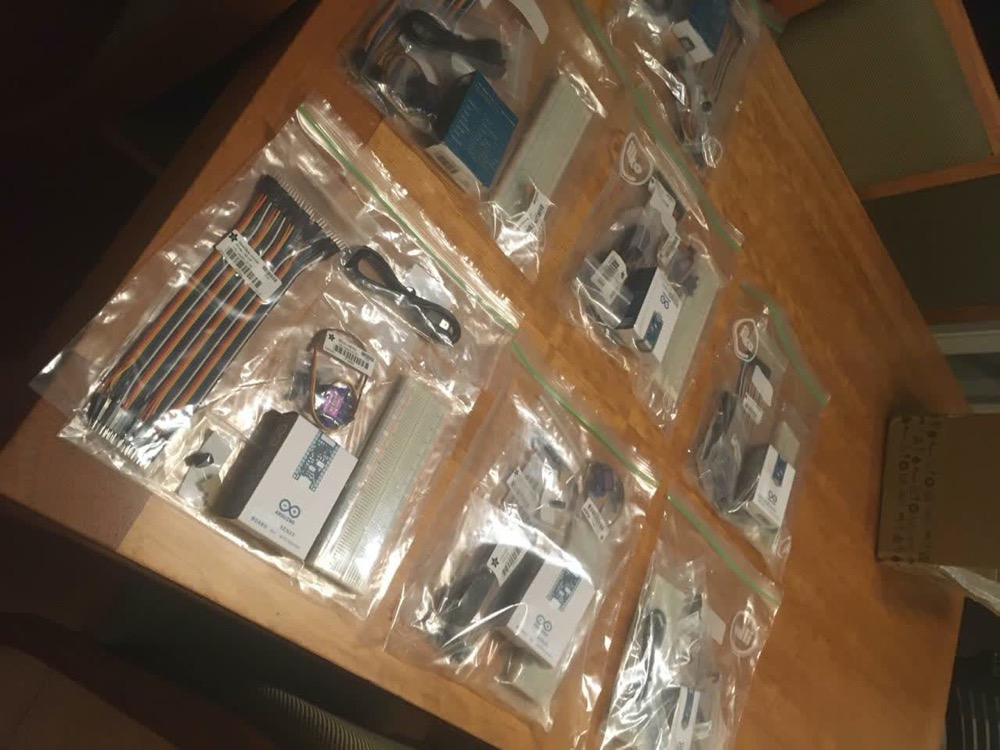
\includegraphics[width=0.75\linewidth,height=0.25\textheight,keepaspectratio]{images/workshop-packages-chile.jpg}
  \caption{Workshop packages for the students in Chile}
  \caption*{Picture by Bernardita Moraga}
  \label{fig:workshop-packages-chile}
\end{figure}

In parallel to the shipping of the materials, the participants were sent instructions via email with links to the project's documentation, in particular to install the Arduino \acrshort{IDE}, the TinyTrainable library, and its dependencies. If students had problems while installing, I helped them over email or videoconferencing. Over the course of teaching the workshops, I updated the installation instructions to make them clearer and updated.

\section{Workshop curriculum}

In the first session, the students make sure their installation of the software is correct. After that, they unbox their materials, and place their Arduino microcontroller on their breadboard. Then they connect it with their USB cable to their computer and upload their first code example, to check that both hardware and software is functioning correctly.

When this is done with success, the students learn about the embedded RGB and proximity sensors used on the color input. Students learn how to capture their own color database, and train their \acrshort{k-NN} algorithm. As an output, first they learn how to read the color classification on their serial port, and then they wire the buzzer to output sounds with different frequencies and durations. The first session concludes with students modifying the code examples, and are encouraged to try to wire and output movement with their servo motor.

The second session focuses on the gesture and speech detection. The students learn how to capture gesture data with their Arduino microcontroller, and then organize it in a formatted database. Then they learn how to use Google Colab for training on the cloud, and discuss the privacy implications of uploading their data to an external server. Since the data they are handling is not compromising, and for time reasons, we use Google Colab, and they learn the alternatives to train these models on their own machine.

The students learn all the steps involved in creating their database, formatting it, training the model, and adapting it for use with their microcontroller. The final part of this session is an overview of the speech recognition of Tiny Trainable Instruments, and they learn strategies for creating their own speech databases, and resources to gather training from external resources.

\section{Workshop feedback}

After the completion of the workshops, I sent the students a Google form to ask for anonymous feedback. The students gave very encouraging reviews that makes me consider this workshop a success, and I hope to teach it again, and expanding it to a semester-long class for college education. 

The students were asked to describe the workshop with one word. They responded: interesting, challenging, fun, innovative, inspiring, didactical, exciting, fun, new, fast-paced, and experimental.

They said that they learned programming fundamentals, the new artistic possibilities that tiny \acrshort{ML} offers, ethical \acrshort{AI}, and algorithmic bias. All of them also reported that they wanted to keep on learning on their own programming, multimedia art, and \acrshort{ML}.

Their favorite aspects of the workshop are the thoughtfulness and usability of the library, its practical and hands-on approach, its way of making \acrshort{ML} more understandable and inviting, the thorough step-by-step explanations, and the joy of learning together with other artists.

The main complaints were that they wished the workshop was longer and in person, and that they wished we could have covered more advanced topics, including how to package the Tiny Trainable Instruments in a more robust platform, instead of a breadboard. Their suggested additions include video tutorials, more code examples and more sessions for the workshop.

\section{Workshop challenges}

As an instructor the main challenge for me was the rhythm of the workshop, mainly because the code examples around 10 minutes to compile. I choreographed the workshop so that students opened a new example, started the compilation, and while it happened we read and studied the code. With this technique, right after the compilation and upload to the microcontroller, we were ready to start using the code example.

My other challenge was to keep the language of the workshops inviting instead of overwhelming. My strategies to foster a positive environment, included sharing  with the students all the issues I had while developing the library, so they could appreciate the labor involved in writing this library and educational materials. I also gave them context about how recently published were the \acrshort{ML} libraries we used, so that they could appreciate the novelty and timing of this project.

A wide array of challenges from the students were reported on the feedback form. Some of them had problems with their hardware, including internet issues or their computers being too slow to download and compile the code examples. Others wished the workshop was presential, so that we could collaborate in person. Some students also thought that the first session was really easy to understand, and with a good pacing, and that the second session was too advanced for them, and that they would rather dedicate this time to learn with more depth the topics presented in the first session.

Did the workshops provide you with new ideas on how to modify the TinyTrainable library in the future? Or new ideas on how to introduce the library to beginners?

what did participants create


what did they find most interesting



The workshop instructions are documented on the docs/ folder of the repository available at \url{https://github.com/montoyamoraga/tiny-trainable-instruments}

Each workshop consists of 2 sessions of 2 hours each, spread over 2 consecutive days.
